\section{Analisi Preliminare}\label{analisipre}

Il sito che viene analizzato in questa relazione, \url{https://www.ticketone.it/}, nasce con lo scopo di vendere tramite Internet biglietti per eventi musicali, di spettacolo, sportivi e culturali.
Questo facilita di molto la procedura di compravendita dei biglietti in quanto gli utenti ne vedono trasparentemente tutte le opzioni di acquisto e i loro costi, potendo scegliere posti a sedere tramite una rappresentazione grafica del posto dove viene effettuato lo spettacolo, vedere i posti rimanenti, ecc.
\par Da una prima vista si capisce facilmente a che tipo di pubblico si rivolge questo sito e quello che vuole vendere.

\subsection{Scelta del nome e dominio}
	
	\`E molto importante per un sito saper scegliere un nome semplice e adeguato in maniera da poter essere ricordato dall'utente e ricordare i servizi presenti al suo interno.
	In questo caso \textit{TicketOne} è un nome molto facile da ricordare in quanto contiene le parole \textit{ticket} e \textit{one}, come per dire che è il primo posto dove poter andare a comprare i propri biglietti.
	\par Come il nome, anche il dominio aiuta gli utenti a ricordare l'indirizzo completo del sito: in questo caso il dominio \textit{.it} è molto facile da ricordare per l'utente finale.
	\par Per evitare omonimie, l'azienda che detiene questa piattaforma ha comprato anche il dominio \textit{.com}, come viene dimostrato dal reindirizzamento che viene effettuato da \url{https://www.ticketone.com/} verso \url{https://www.ticketone.it/}.

\subsection{Posizionamento nei motori di ricerca}

	Andando a cercare ``\textit{vendita biglietti online}'' su \textit{Google}, TicketOne è nella prima posizione, seguita da \url{https://www.eventbrite.it/} e \url{https://www.prontoticket.it/} (Fig.~\ref{posizionamento}).
	\par L'ottimo posizionamento di TicketOne non è dovuto solamente al fatto del nome e del dominio, che sicuramente influiscono in una percentuale molto alta, ma è dato anche dall'uso di tag \textit{meta} e di \textit{keyword} scelte in maniera mirata e intelligente.
	\begin{figure}[hbt]
		\centering
		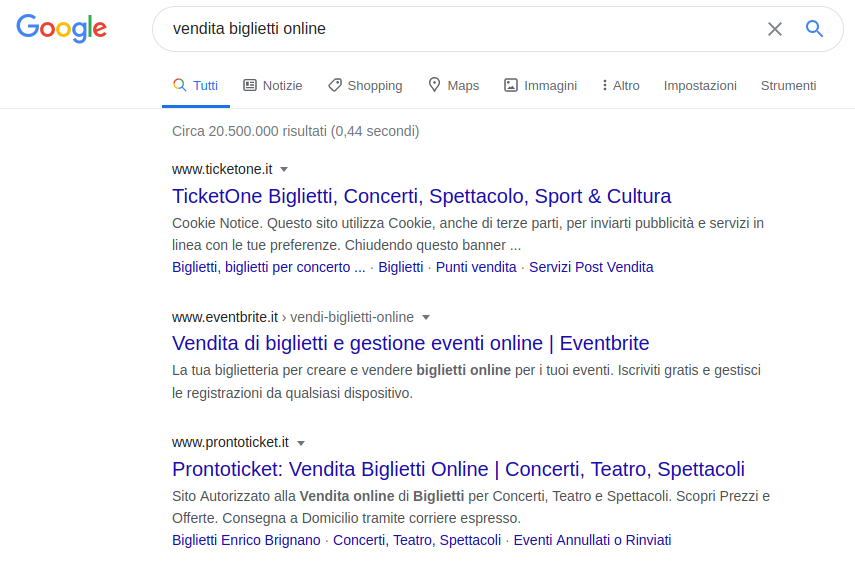
\includegraphics[width=\textwidth]{img/posizionamento.png}
		\caption{Posizionamento di TicketOne nei primi risultati di Google}
		\label{posizionamento}
	\end{figure}

\subsection{Homepage}
	
	Come per molti siti di \textit{e-commerce}, anche in questo caso possiamo paragonare l'homepage di Ticketone (Fig.~\ref{homepage}) alla vetrina di un negozio.
	\begin{figure}[hbt]
	    \centering
	    \includegraphics[width=\textwidth]{img/home.png}
	    \caption{Homepage di TicketOne}
	    \label{homepage}
	\end{figure}
	\par \`E possibile suddividere questa prima pagina in cinque macrosezioni:
	\begin{itemize}[noitemsep]
		\item Header
		\item Barra di ricerca 
		\item Menu laterale
		\item Carosello degli eventi in primo piano
		\item Eventi raggruppati per categoria
	\end{itemize}
	\`E importante notare che quando viene aperto il sito, non compaiono pop up e non ci sono animazioni pesanti che rendono il sito lento da caricare.
	Questa è una nota positiva che invoglia l'utente che non è entrato con uno scopo preciso a restare sulla piattaforma.
	L'unica cosa che viene chiesta all'utente è di accettare o meno l'utilizzo dei cookie.

	\paragraph{Header} Questo si presenta in maniera semplice. 
	Contiene: sulla sinistra il logo del sito e uno slogan, sulla destra il pulsante di accesso al proprio account e il pulsante per poter cambiare lingua e nazione.
	\begin{figure}
		\centering
		
\includegraphics[width=\textwidth]{img/header.png}
		\caption{Header - TicketOne}
		\label{header}
	\end{figure}

	\paragraph{Barra di ricerca} Questa permette di cercare in maniera \textit{dinamica} gli eventi disponibili nel sito, di qualsiasi categoria questi siano.
	\par La ricerca interna di TicketOne viene discussa in dettaglio nella Sez.~\ref{ricerca}.
		
	\paragraph{Menu laterale} Questo permette di navigare il sito spostandosi tra le principali categorie di eventi o località.
	Scorrendo la pagina, il menu contiene altre opzioni come la possibilità di iscriversi alla newsletter, gli eventi consigliati, possibilità di acquistare voucher, ecc.
	\par Il menu laterale viene discusso in dettaglio nella Sez.~\ref{contenav}.
	
	\paragraph{Carosello degli eventi in primo piano} Nonostante sia animato, questo carosello automatico non appesantisce la pagina, né a livello visivo né di caricamento.
	Contiene le miniature dei principali eventi e permette all'utente di capire il servizio principale offerto da questo sito: la vendita di biglietti.
	
	\paragraph{Eventi raggruppati per categoria} Sotto al carosello si intravvede l'inizio della sezione che raggruppa i principali eventi per categoria.
	Queste vengono visualizzate dall'utente solamente quando scorre la pagina.

\subsection{Mappa del sito}
	
	TicketOne non offre una pagina dedicata a mostrare in dettaglio le connessioni tra le pagine del sito e come queste vengono organizzate.
	\par Questa assenza, nonostante possa risultare negativa viene risolta dalla facilità nella navigazione e nella suddivisione chiara delle sezioni, oltre che da una ricerca interna al sito molto esaustiva.

\subsection{Scelta dei colori}
	
	La palette di colori è stata scelta correttamente, in maniera da evitare composizioni e contrasti che stonassero.
	In questo caso il colore predominante di TicketOne è il \textit{blu scuro}, mentre il colore secondario è il \textit{giallo} che, nonostantante non predomini sul bianco dello sfondo, appare nel logo e in vari pulsanti interni al sito.